
\documentclass{article}
\usepackage[a4paper, margin=2cm]{geometry} %Annina style
\usepackage{amsmath}
\usepackage{amssymb}
\usepackage{graphicx}
\usepackage{hyperref}
\usepackage{listings}
\usepackage{xcolor}
\usepackage{tabularx}
\usepackage{array} % for 'm' column type
\usepackage{float} % Include the float package for the H option

\lstset{ 
    language=Python, 
    basicstyle=\ttfamily\small, 
    keywordstyle=\color{blue}, 
    stringstyle=\color{red}, 
    commentstyle=\color{green}, 
    showstringspaces=false,
    numbers=left,
    numberstyle=\tiny\color{gray},
    frame=single,
    breaklines=true
}
\title{Class Notes on GANs Models}
\author{Jack Li}
\date{\today}

\renewcommand{\lstlistingname}{Code}
\begin{document}

\maketitle

\tableofcontents

\section{Introduction}
\label{sec:introduction}
Provide an introduction to GANs and their importance in machine learning.

\section{Basic Math}
\label{sec:basic-math}
\subsection{Probability Theory}
\begin{itemize}
    \item Definitions of probability, random variables, expectation, etc.
\end{itemize}



\subsection{Sampling from a Probability Distribution: Why \( P(x) \, dx \)?}

In continuous probability theory, the **probability density function** (PDF) \( P(x) \) represents the density of the probability at a particular point \( x \). However, the actual probability of the random variable \( X \) falling within a small interval around \( x \), say \( [x, x + dx] \), is given by the product of the PDF at \( x \) and the small interval \( dx \).

\subsubsection{Mathematical Expression}

The probability of \( X \) falling within the interval \( [x, x + dx] \) is approximately:

\[
P(X \in [x, x + dx]) \approx P(x) \, dx
\]

Where:
- \( P(x) \) is the probability density function evaluated at \( x \),
- \( dx \) is an infinitesimally small interval around \( x \).

\subsubsection{Why \( P(x) \, dx \)?}

- The PDF \( P(x) \) by itself does not give the actual probability for any specific value of \( x \), because for continuous random variables, the probability of any single point is zero:
  \[
  P(X = x) = 0 \quad \text{for continuous variables}.
  \]
  
- Instead, the **probability** is found by integrating the PDF over an interval:
  \[
  P(X \in [a, b]) = \int_a^b P(x) \, dx
  \]
  
  For a very small interval \( dx \), the integral simplifies to:
  \[
  P(X \in [x, x + dx]) \approx P(x) \, dx
  \]

This shows that the product \( P(x) \, dx \) gives the probability mass within the small region \( [x, x + dx] \).

\subsubsection{Example of Sampling}

When sampling a value \( x \) from a distribution, the probability that a sample lies within a small range \( [x, x + dx] \) is proportional to \( P(x) \, dx \). For example, in the case of a Gaussian (Normal) distribution, the probability density is given by:

\[
P(x) = \frac{1}{\sqrt{2 \pi \sigma^2}} \exp\left( - \frac{(x - \mu)^2}{2 \sigma^2} \right)
\]

To find the probability of the random variable \( X \) falling within the range \( [x, x + dx] \), we compute:

\[
P(X \in [x, x + dx]) \approx P(x) \, dx
\]\\

\subsection{Standard Sampling (Non-Differentiable)}

In the standard sampling method, we sample directly from a normal distribution, which does not allow gradients to propagate:


\begin{lstlisting}[language=Python]
# Non-differentiable direct sampling
mu = torch.tensor(0.0, requires_grad=True)
sigma = torch.tensor(1.0, requires_grad=True)

# Direct sampling from a normal distribution
z = torch.normal(mu, sigma)

# Loss function
loss = (z - 5) ** 2
loss.backward()  # This breaks the gradient flow
\end{lstlisting}

This will not compute gradients correctly because the sampling is a discrete, non-differentiable operation.

\subsection{Reparameterization Trick (Differentiable)}

In the reparameterization trick, we express the random variable \( z \) as a function of \( \mu \), \( \sigma \), and a noise term \( \epsilon \), which allows backpropagation to compute gradients:

\[
z = \mu + \sigma \cdot \epsilon
\]

\begin{lstlisting}[language=Python]
# Differentiable sampling using reparameterization trick
mu = torch.tensor(0.0, requires_grad=True)
log_sigma = torch.tensor(0.0, requires_grad=True)
sigma = torch.exp(log_sigma)

# Sample epsilon from N(0, 1)
epsilon = torch.randn_like(sigma)

# Reparameterization: z = mu + sigma * epsilon
z = mu + sigma * epsilon

# Loss function
loss = (z - 5) ** 2
loss.backward()  # Gradient flows through mu and sigma
\end{lstlisting}

Here, \( \epsilon \) is sampled from a standard normal distribution \( \mathcal{N}(0, 1) \), and the parameters \( \mu \) and \( \sigma \) can be updated by gradient descent because the whole process is now differentiable.

\subsection{Gumbel-Softmax}

\subsubsection{Definition}

The Gumbel-Softmax trick is a method for sampling from a categorical distribution in a differentiable way. It provides a continuous approximation to a categorical distribution, making it suitable for use in backpropagation.

Let \( \pi_1, \pi_2, \dots, \pi_k \) be the probabilities of each category in a categorical distribution. The Gumbel-Softmax trick works by introducing Gumbel noise \( g_i \) for each category \( i \), sampled from a Gumbel distribution:
\[
g_i = -\log(-\log(u_i)), \quad u_i \sim \text{Uniform}(0, 1)
\]
The continuous approximation to the categorical distribution is given by the softmax function:
\[
y_i = \frac{\exp((\log(\pi_i) + g_i) / \tau)}{\sum_{j=1}^{k} \exp((\log(\pi_j) + g_j) / \tau)}
\]
where \( \tau \) is the temperature parameter controlling the sharpness of the approximation. As \( \tau \to 0 \), the distribution becomes more discrete (closer to one-hot), and as \( \tau \to \infty \), the distribution becomes more uniform.

\subsubsection{Proof of Differentiability}

Let \( \pi = (\pi_1, \pi_2, \dots, \pi_k) \) be the parameter of the categorical distribution. The reparameterization with Gumbel noise is differentiable because:
\[
\frac{\partial y_i}{\partial \pi_j} = \frac{\partial}{\partial \pi_j} \left( \frac{\exp((\log(\pi_i) + g_i) / \tau)}{\sum_{j=1}^{k} \exp((\log(\pi_j) + g_j) / \tau)} \right)
\]
Since \( g_i \) is independent of \( \pi_j \), the function remains differentiable.

\subsection{Concrete Distribution}

\subsubsection{Definition}

The Concrete distribution is similar to the Gumbel-Softmax but is defined for both binary and multinomial distributions. The Concrete distribution for binary random variables introduces a continuous relaxation by using the logistic sigmoid function for binary variables.

For a binary random variable with probability \( p \), the Concrete distribution samples:
\[
z = \frac{\log(p) + g}{\tau}
\]
where \( g \sim \text{Gumbel}(0, 1) \) and \( \tau \) is the temperature parameter. The output \( z \) is passed through the sigmoid function to produce a value between 0 and 1:
\[
y = \sigma(z) = \frac{1}{1 + \exp(-z)}
\]

\subsubsection{Differentiability}

As in the Gumbel-Softmax case, the Concrete distribution is differentiable because the sampling is reparameterized using Gumbel noise, and the final step uses differentiable functions like the softmax or sigmoid.

\subsection{Pros and Cons}

\begin{table}[h!]
\centering
\begin{tabularx}{\textwidth}{| m{3cm} | X | X |}
\hline
\textbf{Method} & \textbf{Pros} & \textbf{Cons} \\
\hline
Gumbel-Softmax & - Differentiable approximation of categorical variables. \newline - Control over discreteness via temperature \( \tau \). \newline - Easy to implement for multiclass problems. & - Approximation error due to continuous relaxation. \newline - Gradients vanish as \( \tau \to 0 \). \newline - Limited to categorical (one-hot) outputs. \\
\hline
Concrete Distribution & - Differentiable for both binary and categorical variables. \newline - More flexibility than Gumbel-Softmax for binary decisions. & - Same vanishing gradient issue as Gumbel-Softmax for low \( \tau \). \newline - Still an approximation of a discrete distribution, not exact. \\
\hline
\end{tabularx}
\caption{Comparison of Gumbel-Softmax and Concrete distribution}
\end{table}

\subsection{Use Cases}

\subsubsection{Gumbel-Softmax}
- **Generative Models**: Used in **Variational Autoencoders (VAEs)** for categorical latent variables, allowing for discrete sampling while maintaining differentiability.
- **Reinforcement Learning**: In policy gradient methods, Gumbel-Softmax can be used for discrete action selection.

\subsubsection{Concrete Distribution}
- **Binary Decision Making**: Useful in models where decisions are binary, like in the **Binary Variational Autoencoder (Binary VAE)**.
- **Binary Latent Variables**: Concrete distributions work well for models with binary latent variables, where a differentiable approximation is required.

\subsection{Equations Summary}

\subsubsection{Gumbel-Softmax Equation}
For categorical variables, the Gumbel-Softmax approximation is given by:
\[
y_i = \frac{\exp((\log(\pi_i) + g_i) / \tau)}{\sum_{j=1}^{k} \exp((\log(\pi_j) + g_j) / \tau)}
\]
where \( g_i \sim \text{Gumbel}(0, 1) \).

\subsubsection{Concrete Distribution Equation}
For binary variables, the Concrete distribution is given by:
\[
z = \frac{\log(p) + g}{\tau}, \quad g \sim \text{Gumbel}(0, 1)
\]
and the relaxed binary sample is:
\[
y = \frac{1}{1 + \exp(-z)}
\]
\subsection{Linear Algebra}
\begin{itemize}
    \item Vectors, matrices, eigenvalues, eigenvectors, etc.
\end{itemize}

\subsection{Optimization}
\begin{itemize}
    \item Gradient descent, stochastic gradient descent, etc.
\end{itemize}

\section{PyTorch Basics}
\label{sec:pytorch-basics}
\subsection{Tensors}
\begin{itemize}
    \item Definition and operations on tensors.
\end{itemize}

\section{PyTorch training gradients}
  \begin{lstlisting}[language=Python, caption=PyTorch training gradients]
  #SECTION: Gradient computation

# Step 1: Define a simple model
model = nn.Linear(1, 1)
optimizer = optim.SGD(model.parameters(), lr=0.01)

# Dummy input and target
input = torch.tensor([[1.0]], requires_grad=True)
target = torch.tensor([[2.0]])

# Step 2: Print the initial parameters
print("Initial parameters:")
for param in model.parameters():
    print(param.data)

# Step 3: Forward pass
output = model(input)
loss = (output - target).pow(2).mean()

# Step 4: Zero the gradients
optimizer.zero_grad()

# Step 5: Backward pass
loss.backward()

# Step 6: Update the parameters
optimizer.step()

# Step 7: Print the parameters after the update
print("\nParameters after one training step:")
for param in model.parameters():
    print(param.data)

\end{lstlisting}

1. \textbf{Initialize Parameters:}\\
   - Assume initial weights \( w \) and bias \( b \) are both 0.\\
   - Model: \( y = wx + b \) \\

2. \textbf{Forward Pass:} \\
   - Compute the output: \( \hat{y} = wx + b \) \\
   - Given input \( x = 1.0 \) and target \( y = 2.0 \): \\
     \[
     \hat{y} = 0 \cdot 1.0 + 0 = 0 \\
     \]

3. \textbf{Compute Loss:} \\
   - Loss function: Mean Squared Error (MSE) \\
     \[
     \text{Loss} = \frac{1}{N} \sum_{i=1}^{N} (\hat{y}_i - y_i)^2 \\
     \]
   - For our single data point: \\
     \[
     \text{Loss} = (0 - 2.0)^2 = 4.0  \\
     \]

4. \textbf{Backward Pass (Gradient Calculation):} \\
   - Compute gradients of the loss with respect to \( w \) and \( b \): \\
     \[
     \frac{\partial \text{Loss}}{\partial w} = 2(\hat{y} - y)x = 2(0 - 2.0) \cdot 1.0 = -4.0 
     \]
     \[
     \frac{\partial \text{Loss}}{\partial b} = 2(\hat{y} - y) = 2(0 - 2.0) = -4.0
     \]

5. \textbf{Parameter Update:}\\
   - Using Stochastic Gradient Descent (SGD) with learning rate \( \eta = 0.01 \): \\
     \[
     w_{\text{new}} = w - \eta \frac{\partial \text{Loss}}{\partial w} = 0 - 0.01 \cdot (-4.0) = 0.04
     \]
     \[
     b_{\text{new}} = b - \eta \frac{\partial \text{Loss}}{\partial b} = 0 - 0.01 \cdot (-4.0) = 0.04
     \]

6. \textbf{Updated Parameters:}\\
   - After one training step, the new parameters are:\\
     \[
     w = 0.04, \quad b = 0.04
     \]

\textbf{Summary}
- Initial parameters: \( w = 0, b = 0 \)
- After one training step: \( w = 0.04, b = 0.04 \)
\subsection{Autograd}
\begin{itemize}
    \item Automatic differentiation in PyTorch.
\end{itemize}
The active selection $gradient.norm(2, dim=1)$ is a PyTorch operation that computes the L2 norm (Euclidean norm) of the $gradient$ tensor along a specified dimension. 
In this case, the dimension specified is $dim=1$.
$$\begin{array}{c}{{\Theta=\!\operatorname*{argmin}_{\Theta}\frac1B\sum_{i=1}^{B}\left[D\Big(z_{i},\Theta\Big)-D\Big(y_{i},\Theta\Big)\right]}}\\ {{+\lambda\!\left(\left\|\frac{\partial D(y,\Theta)}{\partial y}\right\|-1\right)^{2}}}\end{array}$$
Detailed Explanation:\\

\textbf{1. L2 Norm (Euclidean Norm)}: \\

\begin{itemize}
  \item    - The L2 norm of a vector is a measure of its magnitude and is calculated as the square root of the sum of the squares of its components. Mathematically, for a vector \( v \), the L2 norm is given by \( \|v\|_2 = \sqrt{\sum v_i^2} \).\\
  \item    - In PyTorch, the $norm$ function can compute various types of norms, with the L2 norm being specified by the argument $2$. \\
\end{itemize} 

\textbf{2. Dimension Specification ($dim=1$):} \\

   \begin{itemize}
     \item    - The $dim$ argument specifies the dimension along which the norm is computed. In a multi-dimensional tensor, this allows you to compute norms along specific axes. \\
     \item    - For example, if $gradient$ is a 2D tensor (matrix) with shape $[batch size, num features]$, setting $dim=1$ means that the norm is computed for each row independently.
   This results in a tensor of shape $[batch size]$, where each element is the L2 norm of the corresponding row in the original tensor. \\

   \end{itemize}

\begin{lstlisting}[language=Python, caption=PyTorch gradient sampling example]
# Define the sampling function
def sample_function(x):
    return torch.sin(x)


# NOTE: Generate sample points with requires_grad=True, and need requires_grad=True
# Generate sample points with requires_grad=True
x = torch.tensor(
    np.linspace(0, 2 * np.pi, 100), dtype=torch.float32, requires_grad=True
)

# Define f by sampling from the sample_function
f = sample_function(x)

# Compute the gradient of f with respect to x
grad = torch.autograd.grad(outputs=f, inputs=x, grad_outputs=torch.ones_like(f))

print(f"The gradient of f(x) = sin(x) at x = {x} is {grad[0]}")

\end{lstlisting}

\subsection{Building Neural Networks}
\begin{itemize}
    \item Layers, activation functions, loss functions, etc.
\end{itemize}


\begin{figure}[H]
    \centering
    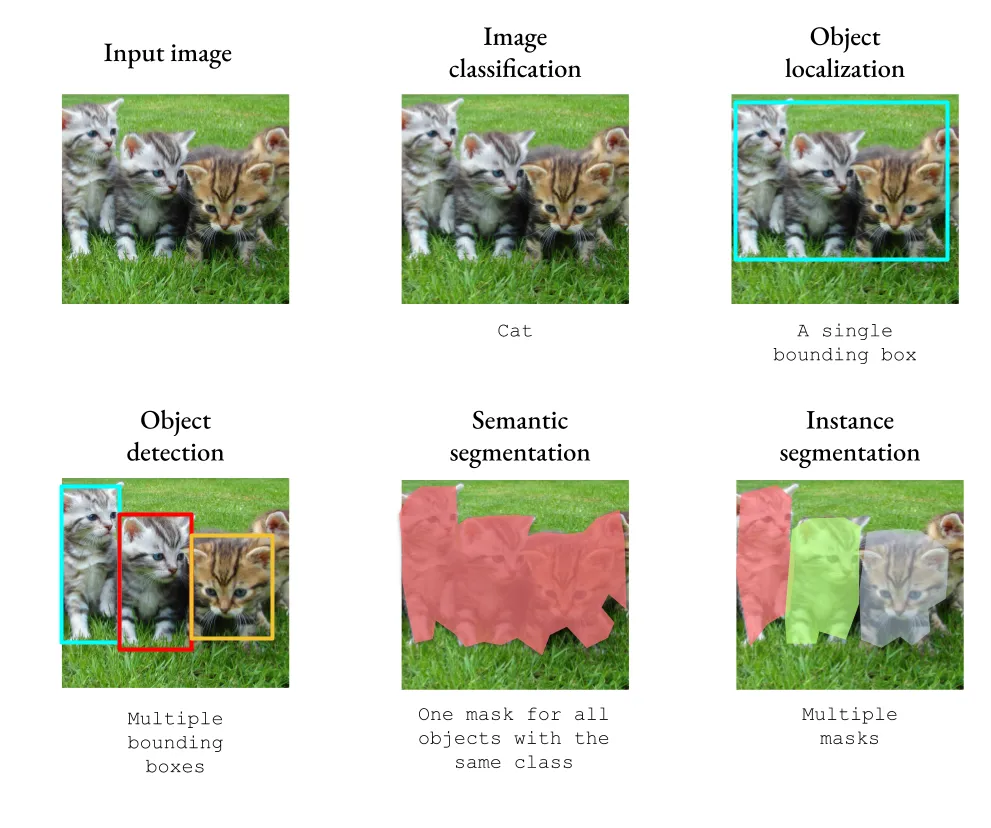
\includegraphics[width=\linewidth]{../fig/segmentation_explain.png} % Replace with the path to your image
    \caption{An example image illustrating segmentation.}
    \label{fig:example}
\end{figure}

\subsection{Loss Functions}

--- PyTorch Conv2d Equation \\

The output size of a Conv2d layer can be calculated using the following equation:

\[ \text{Output Size} = \left\lfloor \frac{\text{Input Size} + 2 \times \text{Padding} - \text{Kernel Size}}{\text{Stride}} \right\rfloor + 1 \]

Where:
- \(\text{Input Size}\) is the size of the input feature map (height or width).
- \(\text{Padding}\) is the number of zero-padding added to both sides of the input.
- \(\text{Kernel Size}\) is the size of the convolution kernel (height or width).
- \(\text{Stride}\) is the stride of the convolution.

PyTorch ConvTranspose2d Equation\\

The output size of a ConvTranspose2d (transposed convolution) layer can be calculated using the following equation:

\[ \text{Output Size} = (\text{Input Size} - 1) \times \text{Stride} - 2 \times \text{Padding} + \text{Kernel Size} + \text{Output Padding} \]

Where:
- \(\text{Input Size}\) is the size of the input feature map (height or width).
- \(\text{Stride}\) is the stride of the convolution.
- \(\text{Padding}\) is the number of zero-padding added to both sides of the input.
- \(\text{Kernel Size}\) is the size of the convolution kernel (height or width).
- \(\text{Output Padding}\) is the additional size added to the output (usually used to ensure the output size matches a specific value).


\section{GANs Models}
\label{sec:gans-models}
\subsection{Basic GAN}
\begin{itemize}
    \item Architecture: Generator and Discriminator.
    \item Loss functions: Minimax game.
    \item Training process.
\end{itemize}

\subsection{DCGAN}
\begin{itemize}
    \item Architecture: Convolutional layers.
    \item Improvements over basic GAN.
    \item Training tips.
\end{itemize}

\subsection{WGAN}
\begin{itemize}
    \item Wasserstein distance.
    \item Critic network.
    \item Gradient penalty.
\end{itemize}

\subsection{CycleGAN}
\begin{itemize}
    \item Architecture: Cycle consistency loss.
    \item Applications: Image-to-image translation.
\end{itemize}

% Add more GANs models sections as needed

\section{Conclusion}
\label{sec:conclusion}
Summarize the key points and discuss future directions.

\end{document}
